\documentclass[12pt]{report}

\usepackage[T1]{fontenc}
\usepackage[utf8]{inputenc}
\usepackage{graphicx}

\begin{document}
 
\begin{center}
{\Huge Circuitos de control de voltaje y corriente con tiristores}
\end{center}
\begin{center}

\includegraphics[scale=1]{../../../../Downloads/upzmg.jpg} 
\end{center} 
{\Huge Enesto Alonso Partida López\\Osmar de Jesus Cruz Ramirez\\ Universidad Politecnica De La Zona Metropolitana De Guadalajara\\ Mecatronica 4 A\\ Septiembre-diciembre 2019}
\date{3 de noviembre  2019}
 
\newpage

{\huge \textbf{INTRODUCCION:}\\}\\


{\large Mediante la utilización de triac o bien tiristores se pretende controlar la intensidad de una lampara la cual contara con un foco, así como conocer el funcionamiento de los diodos diac, los cuales nos permitirán el paso de corriente para lograr encender el foco a una cierta intensidad.}\\
 

{\huge \textbf{OBJETIVO}\\}\\


{\large Lograr que el foco quede completamente iluminado, así como también lograr que este se apague por completo al regular la resistencia del circuito con un potenciómetro }\\



{\huge \textbf{MARCO TEORICO}\\}\\


{\large DIAC: Control de potencia en corriente alterna (AC)\\
El DIAC es un diodo de disparo bidireccional, especialmente diseñado para disparar TRIACs y Tiristores (es un dispositivo disparado por tensión).El TRIAC tiene dos terminales: MT1 y MT2. Ver el diagrama. El DIAC se comporta como dos diodos zener conectados en serie, pero orientados en formas opuesta. La conducción se da cuando se ha superado el valor de tensión del zener que está conectado en sentido opuesto. El DIAC normalmente no conduce, sino que tiene una pequeña corriente de fuga. La conducción aparece cuando la tensión de disparo se alcanza.\\\\ \\
\begin{center}
\begin{figure}[hbtp]
\caption{Diac}
\centering
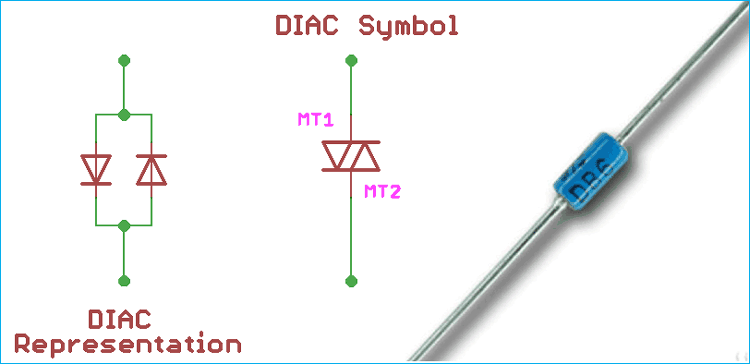
\includegraphics[scale=.5]{../../../../Downloads/descragas/diac.png}
\end{figure}
\end{center}
{\large Tiristor\\El tiristor es un semiconductor de potencia que se utiliza como interruptor, ya sea para conducir o interrumpir la corriente eléctrica, a este componente se le conoce como de potencia por que se utilizan para manejar grandes cantidades de corriente y voltaje, a comparación de los otros semiconductores que manejan cantidades relativamente bajas.
Cuando se habla de tiristores comúnmente se cataloga al tiristor como un SRC (silicon controlled rectifier), pero esto no es del todo correcto ya que este tipo es el más popular y conocido pero no es el único que existe. }}
\begin{center}
\begin{figure}[hbtp]
\centering
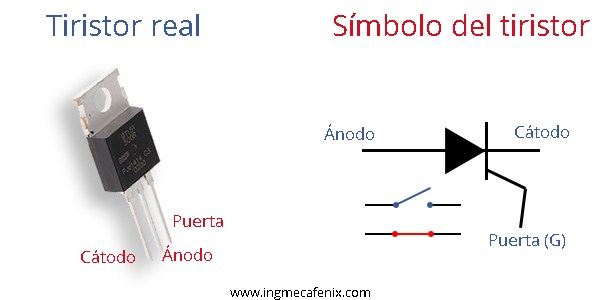
\includegraphics[scale=0.5]{../../../../Downloads/descragas/tiristor.jpg}
\caption{Tiristor }
\end{figure}

\end{center}
\newpage

{\huge \textbf{MATERIALES}\\}\\


\begin{enumerate}
\item Protoboard
\item Potenciometro de 100k
\item Foco
\item Resistencias
\item Base para foco
\item Diac
\item Fuente de Voltaje
\item Clabe Para Protoboard
\item Caimanes
\item tiristores
\item Capacitor a 100V
\end{enumerate}


{\huge \textbf{Desarrollo}\\}\\
{\large \begin{enumerate}
\item Se comenzará con el armado del circuito como se presenta en el diagrama, cuidando dejar el capacitor conectado bien porque de lo contrario puede ocasionar fallas y explotar. 
\item Cuando se termine de armar el circuito será necesario conectar el foco junto con su base y la corriente la cual será de 120V para lo cual será necesario usar una clavija y caimanes para conectarse.
\item Posteriormente es necesario ajustar el potenciómetro para logra que el foco aumente y disminuya su intensidad, es importante que durante el procedimiento no se toque ningún componente ya que puedes sufrir descargas y a su vez es importante aislar los cables que conducirán la corriente de 120V.
\item En dado caso que no se logre apagar por completo el foco, será necesario colocar una resistencia más grande para evitar el paso de la corriente, además, será un juego de quitar y poner resistencias para lograr el objetivo, esto se tendrá que ir probando cada  que se cambie una resistencia.
\end{enumerate}}

{\huge \textbf{Resultados obtenidos}\\}\\
{\large Se tuvo que colocar una resistencia diferente a la plateada en el diagrama la cual fue de 570k Ohms a la cual a su vez se le conecto en serie una resistencia más pequeña de 10k Ohms con la cuales se logró que el foco perdiera toda su luminosidad y a la vez lograr que el foco encendiera con una intensidad no tan luminoso como cuando se tiene conectado directamente sin resistencias, pero si una luminosidad que es aceptable.}

{\huge \textbf{Conclusión}\\}\\
{\large Este tipo de circuito se encuentra presente en lugares donde es necesario cambiar la iluminación del cuarto donde se encuentre, a la vez funciona como un interruptor por lo cual se sustituye, pero se tiene que tener cuidado con las resistencias y el capacitor ya que pueden provocar que el circuito deje de funcionar, también es muy importante que en cada circuito que se utilicen grades voltajes, es necesario recubrir los cables para evitar cualquier accidente, es muy interesante este tipo de circuitos sobre todo porque es necesario calcular tanto una resistencia para lograr una intensidad muy luminosa así como para lograr que el foco se apague por lo cual es un poco mas tedioso a la habitual..}
\newpage
{\huge \textbf{Bibliografia:}\\}\\
@online{Electronica Unicrom,
author = {Frank Mecafenix },
title = {Ingeniería Mecafenix},
year = {2016},
url = {https://www.ingmecafenix.com/electronica/puente-h-control-motores/},
OPTsubtitle = {La enciclopedia de la ingeniería},
OPTlanguage = {Español},
OPTversion = {1},
OPTdate = {21},
OPTmonth = {6},
OPTurldate = {https://www.ingmecafenix.com/electronica/puente-h-control-motores/},
}
\\
@online{Electrónica Unicrom,
author = {ELECTRÓNICA PARA EL AFICIONADO Y EL EXPERTO},
title = {DIAC – Diodo de disparo bidireccional – Diode alternative current},
year = {2016},
url = {https://unicrom.com/diac-diodo-disparo-bidireccional/},
OPTlanguage = {español},

}


\end{document}